\documentclass[14pt]{extarticle}

\usepackage[russian]{babel}
\usepackage[utf8]{inputenc}
\usepackage[T2A]{fontenc}
\usepackage{amsfonts}
\usepackage{amsmath}
\usepackage[
	left 	= 	30	mm,
	right 	=	15	mm,
	top 	=	20	mm,
	bottom 	=	20	mm,
]{geometry}

\setlength{\parindent}{1.25 cm}
\usepackage{indentfirst}

\usepackage[toc,page]{appendix}

\renewcommand{\baselinestretch}{1.5}

\usepackage{titlesec}

\titleformat{\section}
  {\normalfont\fontsize{14}{14}\bfseries}{\thesection}{1em}{}

\titleformat{\subsection}
  {\normalfont\fontsize{14}{14}\bfseries}{\thesubsection}{1em}{}

\usepackage[intoc]{nomencl}
\renewcommand{\nomname}{Обозначения и сокращения}
\makenomenclature
	
%%% Математика

% Шрифты для математики
\usepackage{amsmath}
\usepackage{amsfonts}
\usepackage{amssymb}
\usepackage{cancel}
\usepackage{mathrsfs}
\usepackage{mathtools}
\usepackage{upgreek}
\usepackage{xfrac}


%%% Иллюстрации
\usepackage{graphicx}
\usepackage{subcaption}
\usepackage{wrapfig}
\usepackage[export]{adjustbox}
%\graphicspath{{./img/}}
				
%Подписи
\usepackage		[margin		= 10	pt,
%					font		= footnotesize, 
					labelfont	= bf, 
					labelsep	= endash, 
					labelfont	= bf,
%					textfont	= sl,
					margin		= 0 	pt,  
					aboveskip 	= 4		pt, 
					belowskip 	= -6	pt,
					figurename= Рисунок] {caption}
\usepackage		[margin		= 10	pt,
					font		= footnotesize, 
					labelfont	= bf, 
					labelsep	= endash, 
					labelfont	= bf,
					textfont	= sl,
					margin		= 0 	pt,  
					aboveskip 	= 4		pt, 
					belowskip 	= 6	pt]	{subcaption}

%%% Insert pdf pages
\usepackage[final]{pdfpages}


%%% Color highlight
\usepackage{xcolor}


\begin{document}
%	\includepdf[pages=-]{titlesheet.pdf}
	
	\setcounter{page}{2}
	% Аннотация
	\begin{abstract}
		Дерево отрезков - это мощная структура данных, которая позволяет эффективно решать множество задач различных тематик. Данный диплом посвящен построению оптимального дерева в случае известного распределения вероятностей запросов. Было предложено как точное решение, так и асимптотически оптимальное приближенное решение. На наших тестах приближенное решение показало достаточно небольшое ухудшение по сравнению с оптимальным.
	\end{abstract}
	\newpage
	
	% Содержание
	\tableofcontents
	\newpage
	
	\section{Введение}
	\subsection{Определения}

Пусть дан массив из $n$ элементов. \\
\textbf{Дерево отрезков} - это двоичное дерево, в котором:

\begin{itemize}
    \item Есть $n$ листьев, соответствующих отрезкам единичной длины
    \item Есть вершины с двумя сыновьями. Правый сын соответствует отрезку,
    следующему сразу за отрезком левого сына. Вершина соответствует
    объединению отрезков сыновей
    \item Корень дерева соответствует всему массиву (отрезку $[1; n]$).
\end{itemize}

\textbf{Запрос сверху} на отрезке $[L, R]$ начинается в корне.
Если сейчас рассматривается вершина, отрезок которой не лежит полностью в
отрезке $[L, R]$, то запрос рекурсивно вызывается от тех сыновей, отрезки которых
пересекаются с $[L, R]$. Иначе рекурсивных вызовов от сыновей не происходит.
В обоих случаях вершина считается посещенной и в ней выполняются какие-то
действия, специфичные для запроса.

Пример запроса сверху указан на рисунке \ref{fig:segtree_example}. Здесь дерево отрезков на пяти элементах и запрос на отрезке $[2;4]$. Будет посещено пять выделенных вершин.

\begin{figure}[hbt!]
    \centering
    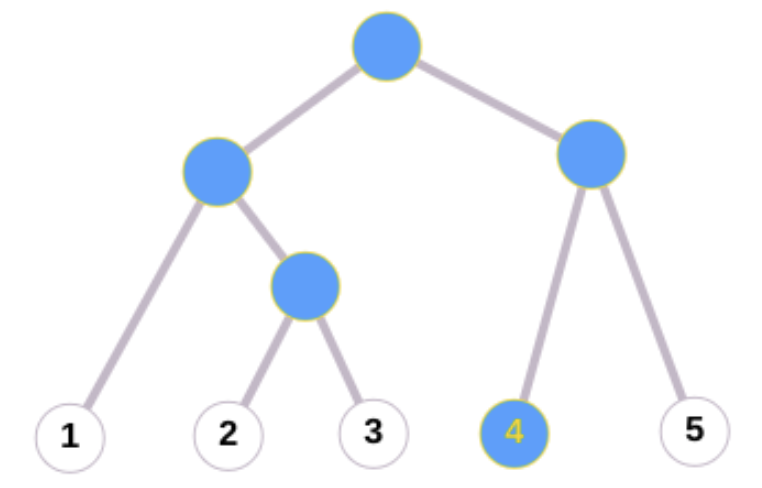
\includegraphics[scale=0.28]{images/segtree_example.png}
    \caption{Пример запроса к дереву отрезков}
    \label{fig:segtree_example}
\end{figure}

\subsection{Постановка задачи}

\textbf{Дано:} Распределение вероятностей на запросах-отрезках границами из $[1; n]$

\textbf{Необходимо:} построить дерево отрезков, для которого минимально среднее
количество посещенных вершин при запросах сверху.

Интересует как точное решение за как можно более лучшую асимптотику, так и
приближенное за сложность нахождения $O(n + S)$ или $O(n + S \log S)$, где $S$ -
количество отрезков с ненулевой вероятностью

\subsection{Мотивация}

Дерево отрезков - это мощная структура данных, которая позволяет решать большое количество задач. 
Если дан массив $a$ из $n$ элементов, то она позволяет эффективно:

\begin{itemize}
    \item Отвечать на запросы $f(a_L, f(\dots, a_R)\dots)$, где $f$ - произвольная ассоциативная функция с двумя аргументами
    \item Изменять элементы $a_L,\dots,a_R$ для некоторых типов изменений
\end{itemize}

Пример: запросы суммы/минимума на подотрезке массива и прибавления числа ко всем элементам подотрезка массива.

Обычно для этого в каждой вершине дерева отрезков хранится значение функции на соответствующем подотрезке массива и информация о том, нужно ли применить какие-то отложенные изменения к сыновьям данной вершины.

Запросы на расчёт функции находятся с помощью запроса сверху и объединения результатов для посещенных вершин. Запросы на изменение тоже совершаются с помощью запросов сверху, для посещенных вершин происходит изменение информации в них нужным образом.

Если для каждой вершины дерева с двумя сыновьями её отрезок разбивается примерно пополам и каждой половине соответствуют её сыновья, то можно показать, что при запросе сверху посещается $O(\log n)$ вершин.

При этом большое количество задач различных тематик можно свести к запросам на подотрезках массива. Примеры таких задач:

\begin{itemize}
    \item Для дерева из $n$ вершин после препроцессинга за $O(n)$ можно отвечать на запросы минимального общего предка за $O(\log n)$
    \item Для строки из $n$ символов после построения суффиксного массива и дополнительного препроцессинга за $O(n)$ можно находить длину наибольшего общего префикса двух любых её подстрок
    \item Если нам дано $n$ прямоугольников на плоскости со сторонами, параллельными осям координат, то можно найти площадь их объединения за $O(n \log n)$
\end{itemize}

Как уже было сказано, если для каждой вершины разбивать её подотрезок на две равные части, то сложность запроса к дереву отрезков $O(\log n)$. Но нам может быть известно распределение вероятностей запросов, и в таком случае можно построить более оптимальное дерево. Таким образом решение задачи, поставленной в дипломе, может привести к ускорению на большом классе задач и может представлять не только теоретический, но и практический интерес.

Кроме того надо заметить, что данный диплом далеко не первый, посвященный вопросу построения оптимальных структур данных при известном распределении вероятностей запросов. В частности, смежная задача построения статически оптимального дерева поиска хорошо изучена, её результаты будут использоваться в дальнейшем.
    \newpage
    
    \section{Обзор смежной задачи}
    \subsection{Определения и постановка задачи}

Хорошо изучена похожая задача нахождения статически оптимального дерева поиска.

Постановка этой задачи такова: есть множество из $n$ различных упорядоченных элементов и вероятности:

\begin{itemize}
    \item $A_1,\dots,A_n$, что запрос будет с значением, равным соответствующему элементу множества
    \item $B_0,\dots,B_n$, что запрос будет лежать до первого элемента, либо между двумя элементами, либо после последнего
\end{itemize}
  
Необходимо найти дерево поиска на данном множестве такое, что среднее количество посещенных вершин при запросах будет минимально.

Дерево поиска - это двоичное дерево такое, что

\begin{itemize}
    \item Есть $n$ вершин, в которых стоят различные значения из данного множества
    \item Если в вершине стоит число $x$, то у всех вершин в её левом поддереве значения меньше чем $x$, в правом поддереве больше чем $x$
\end{itemize}
  
Запрос к дереву поиска выглядит таким образом. Он начинается в корне. Если число из запроса меньше, чем число в текущей вершине, то переходим в её левого сына. Если больше, то в правого. Иначе, а также если мы попытались пойти в несуществующую вершину, запрос завершается.

\subsection{Решения}

В статье \cite{knuth71} было получено точное решение за $O(n^2)$ времени и памяти.

Идея такова - можно найти $dp_{L, R}$ - оптимальное среднее количество посещенных вершин, если дерево построено на значениях с $L$ по $R - 1$. Например, для случая нулевых $B_i$ верно, что

\begin{itemize}
    \item $dp_{L, L} = 0$
    \item $dp_{L, R} = A_L + \dots + A_{R - 1} + \min \limits_{L \leqslant m < R} {dp_{L, m} + dp_{m + 1, R}}$
\end{itemize}
  
Это верно, так как на каждом шаге выбирается элемент в корне поддерева, а затем задачу можно свести к задачам для левого и правого поддерева. При этом каждый запрос пройдёт через корень поддерева и его вероятность нужно прибавить.
  
Так как $dp_{L, R}$ зависит только от значений $dp$ для меньших по длине отрезков, то если перебирать отрезки по неубыванию, $dp_{L, R}$ можно найти за $O(n^3)$ времени. Дальше в статье доказывалось, что в данном случае можно оптимизировать решение до $O(n^2)$ времени.

В статье \cite{mehlhorn1975} было получено приближенное решение за $O(n)$ времени. Идея такова - на каждом шаге выбирать такое значение в корне поддерева, что суммы вероятностей запросов в подзадачах для левого и правого поддерева как можно более близки друг к другу, после этого рекурсивно запустить решение для поддеревьев.

Было показано, что $0.63H \leqslant P_{opt} \leqslant P_{approx} \leqslant 2 + 1.44H$, где $H$ - энтропия распределения вероятностей, $P_{opt}$ - среднее количество посещенных вершин в оптимальном решении, $P_{approx}$ - в приближенном. Таким образом, приближенное решение не хуже оптимального более чем в константу раз, где константу можно оценить сверху как $2.29$

В статье \cite{garsia1977} было приведено точное решение за $O(n \log n)$ времени для важного случая, когда вероятности $A_i$ равны нулю.

В статье \cite{yao1980} было приведено обобщение того, когда точные решения за $O(n^3)$ времени могут быть соптимизированы до $O(n^2)$
    \newpage
    
    \section{Точное решение за $O(n^3+S)$ времени и $O(n^2)$ памяти}
    Здесь будет точное решение TODO
    \newpage
    
    \section{Асимптотически оптимальное приближенное решение}
    Здесь будет приближенное решение TODO
    \newpage

	\section{Заключение}
	Было найдено точное решение задачи за $O(n^3 + S)$ и асимптотически оптимальное приближенное решение. Также были доказаны два неравенства, почти совпадающие с теми, которые используются для доказательства существования решения за $O(n^2)$ для класса задач.

Все найденные решения были написаны и проверены на достаточно небольших случайных тестах, на которых у приближенного решения константа ухудшения ответа по сравнению с оптимальным оказалась достаточно невелика, чтобы данное решение могло иметь не только теоретический, но и практический интерес.

Возможные улучшения - доказательство лучшей константы у приближенного решения и нахождение еще более оптимального точного решения.
	\newpage
	
	% Список литературы
	\begin{thebibliography}{9} 
	\addcontentsline{toc}{section}{Список литературы}
	\bibitem{knuth71} Knuth, Donald E, \emph{"Optimum binary search trees"}. Acta Informatica, 1971.
	\bibitem{mehlhorn1975} Mehlhorn, Kurt, \emph{"Nearly optimal binary search trees"}. Acta Informatica, 1975.
	\bibitem{garsia1977} Garsia, Adriano M, Wachs, Michelle L, \emph{ new algorithm for minimum cost binary trees"}. SIAM Journal on Computing, 1977.
	\bibitem{yao1980} F. Frances Yao, \emph{"Efficient Dynamic Programming Using Quadrangle Inequalities"}. STOC, 1980.
\end{thebibliography}
\end{document}
